\documentclass[tikz, border=10pt]{standalone}
\usepackage{amsmath}
\usepackage{tikz}
\usetikzlibrary{decorations.pathmorphing, arrows.meta, calc, backgrounds}

\definecolor{navybg}{RGB}{13,27,42}
\definecolor{source1col}{RGB}{0,220,255}
\definecolor{source2col}{RGB}{255,165,0}
\definecolor{labelcol}{RGB}{220,220,220}
\definecolor{plotbg}{RGB}{25,40,60}
\definecolor{axiscol}{RGB}{180,180,180}
\definecolor{fockcol}{RGB}{180,100,255}

\begin{document}
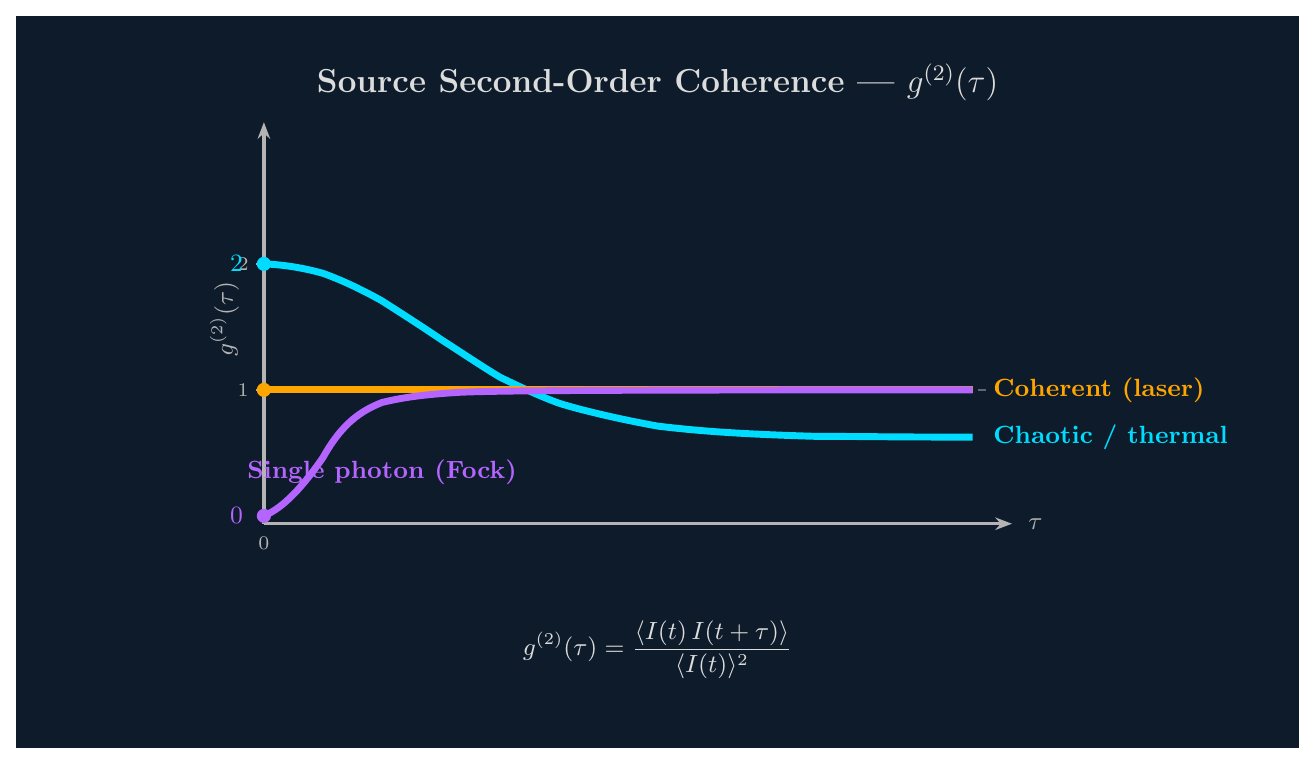
\begin{tikzpicture}[
    background rectangle/.style={fill=navybg},
    show background rectangle,
    arr/.style={-{Stealth[length=6pt]}, line width=1.2pt},
]

\path[use as bounding box] (0,0) rectangle (16,9);

% ════════════════════════════════════════════════════════
% 0. TITLE
% ════════════════════════════════════════════════════════
\node[text=labelcol, font=\large\bfseries] at (8.0, 8.3)
    {Source Second-Order Coherence \textemdash\ $g^{(2)}(\tau)$};

% ════════════════════════════════════════════════════════
% 1. PLOT: g^(2)(τ) for three source types
% ════════════════════════════════════════════════════════
\coordinate (PLOT) at (3.0, 2.8);

% Axes
\draw[arr, axiscol] ($(PLOT)+(0,-0.1)$) -- ($(PLOT)+(9.5,-0.1)$);
\draw[arr, axiscol] ($(PLOT)+(0,-0.1)$) -- ($(PLOT)+(0, 5.0)$);
\node[text=axiscol, font=\small] at ($(PLOT)+(9.8,-0.1)$) {$\tau$};
\node[text=axiscol, font=\small, rotate=90] at ($(PLOT)+(-0.5, 2.5)$) {$g^{(2)}(\tau)$};
\node[text=axiscol, font=\scriptsize] at ($(PLOT)+(0.0,-0.35)$) {$0$};

% y-axis ticks
\draw[axiscol, line width=0.6pt] ($(PLOT)+(-0.1, 1.6)$) -- ($(PLOT)+(0.1, 1.6)$);
\node[text=axiscol, font=\scriptsize, left=2pt] at ($(PLOT)+(0, 1.6)$) {$1$};
\draw[axiscol, line width=0.6pt] ($(PLOT)+(-0.1, 3.2)$) -- ($(PLOT)+(0.1, 3.2)$);
\node[text=axiscol, font=\scriptsize, left=2pt] at ($(PLOT)+(0, 3.2)$) {$2$};

% Dashed reference line at g^(2) = 1
\draw[axiscol, line width=0.8pt, dashed, opacity=0.5]
    ($(PLOT)+(0.0, 1.6)$) -- ($(PLOT)+(9.3, 1.6)$);

% ── Chaotic/thermal light (cyan): g^(2)(τ) = 1 + exp(-(τ/τ_c)^2)
% y_plot = 1.6 + 1.6*exp(-(x/3)^2), τ_c = 3 plot units
% x=0:3.20, x=0.5:3.15, x=1:2.99, x=1.5:2.73, x=2:2.41, x=2.5:2.08,
% x=3:1.76, x=3.5:1.52, x=4:1.35, x=5:1.14, x=6:1.04, x=7:1.01
\draw[source1col, line width=2.5pt]
    ($(PLOT)+(0.0,  3.20)$)
    .. controls ($(PLOT)+(0.25, 3.19)$) and ($(PLOT)+(0.5,  3.15)$) ..
    ($(PLOT)+(0.75, 3.08)$)
    .. controls ($(PLOT)+(1.0,  2.99)$) and ($(PLOT)+(1.25, 2.87)$) ..
    ($(PLOT)+(1.5,  2.73)$)
    .. controls ($(PLOT)+(1.75, 2.57)$) and ($(PLOT)+(2.0,  2.41)$) ..
    ($(PLOT)+(2.25, 2.24)$)
    .. controls ($(PLOT)+(2.5,  2.08)$) and ($(PLOT)+(2.75, 1.91)$) ..
    ($(PLOT)+(3.0,  1.76)$)
    .. controls ($(PLOT)+(3.25, 1.64)$) and ($(PLOT)+(3.5,  1.52)$) ..
    ($(PLOT)+(3.75, 1.43)$)
    .. controls ($(PLOT)+(4.0,  1.35)$) and ($(PLOT)+(4.5,  1.23)$) ..
    ($(PLOT)+(5.0,  1.14)$)
    .. controls ($(PLOT)+(5.5,  1.08)$) and ($(PLOT)+(6.0,  1.04)$) ..
    ($(PLOT)+(7.0,  1.01)$)
    .. controls ($(PLOT)+(7.5,  1.01)$) and ($(PLOT)+(8.0,  1.00)$) ..
    ($(PLOT)+(9.0,  1.00)$);

% ── Coherent light / laser (orange): g^(2)(τ) = 1 for all τ
\draw[source2col, line width=2.5pt]
    ($(PLOT)+(0.0, 1.6)$) -- ($(PLOT)+(9.0, 1.6)$);

% ── Single-photon / Fock state (purple): g^(2)(0) = 0, rises to 1
% y_plot = 1.6*(1 - exp(-(τ/τ_c)^2)), τ_c = 2 plot units
% x=0:0.00, x=0.5:0.38, x=1:1.32, x=1.5:2.12, x=2:2.46 (wait — should rise from 0 to 1.6)
% y = 1.6*(1 - exp(-(x/2)^2)):
% x=0:0.00, x=0.5:0.38, x=1:1.32, x=1.5:2.13, wait that exceeds 1.6
% Correct: x=0:0.00, x=0.5:0.38, x=1:1.19, x=1.5:1.44, x=2:1.54, x=3:1.59, x=4:1.60
\draw[fockcol, line width=2.5pt]
    ($(PLOT)+(0.0,  0.00)$)
    .. controls ($(PLOT)+(0.25, 0.10)$) and ($(PLOT)+(0.5,  0.38)$) ..
    ($(PLOT)+(0.75, 0.74)$)
    .. controls ($(PLOT)+(1.0,  1.19)$) and ($(PLOT)+(1.25, 1.34)$) ..
    ($(PLOT)+(1.5,  1.44)$)
    .. controls ($(PLOT)+(1.75, 1.50)$) and ($(PLOT)+(2.0,  1.54)$) ..
    ($(PLOT)+(2.5,  1.57)$)
    .. controls ($(PLOT)+(3.0,  1.59)$) and ($(PLOT)+(4.0,  1.60)$) ..
    ($(PLOT)+(9.0,  1.60)$);

% ── Source labels (right side)
\node[text=source1col, font=\small\bfseries, right=4pt] at ($(PLOT)+(9.0, 1.00)$)
    {Chaotic / thermal};
\node[text=source2col, font=\small\bfseries, right=4pt] at ($(PLOT)+(9.0, 1.60)$)
    {Coherent (laser)};
\node[text=fockcol, font=\small\bfseries, right=4pt] at ($(PLOT)+(9.0, 1.56)$) {};

% ── g^(2)(0) annotations
\node[text=source1col, font=\small, left=4pt] at ($(PLOT)+(0.0, 3.20)$) {$2$};
\node[text=source2col, font=\small, left=4pt] at ($(PLOT)+(0.0, 1.60)$) {};
\node[text=fockcol,   font=\small, left=4pt] at ($(PLOT)+(0.0, 0.00)$) {$0$};

% Dots marking g^(2)(0) for each source on y-axis
\fill[source1col] ($(PLOT)+(0.0, 3.20)$) circle (0.09);
\fill[source2col] ($(PLOT)+(0.0, 1.60)$) circle (0.09);
\fill[fockcol]    ($(PLOT)+(0.0, 0.00)$) circle (0.09);

% Single-photon label (below the curve, not clashing with laser)
\node[text=fockcol, font=\small\bfseries] at ($(PLOT)+(1.5, 0.55)$)
    {Single photon (Fock)};

% ════════════════════════════════════════════════════════
% 2. BOTTOM EQUATION
% ════════════════════════════════════════════════════════
\node[text=labelcol, font=\small, align=center] at (8.0, 1.1)
    {$g^{(2)}(\tau) = \dfrac{\langle I(t)\,I(t+\tau)\rangle}{\langle I(t)\rangle^2}$};

\end{tikzpicture}
\end{document}
